% !TEX root = ../TV-Denoising.tex

\section{Support stablity for nonsmooth convex sets}\label{sec:no_source_cond}

The theory developed in Sections~\ref{sec:proplev}, \ref{sec:extended} and \ref{sec:stab_extended_spt} relies on the existence of a subgradient of the total variation for $f$ in the $L^2$ topology (source condition). As natural as it may seem, this hypothesis does not always hold even for simple functions (like the indicator function of a square). In some cases, however, there is a natural limit for the dual certificates $\vlao$ when considering another topology.

 This section studies the case of a union $\Omega$ of disjoint convex subsets of $\RR^2$ which are sufficiently far apart. If their boundary is not smooth enough, the source condition is not satisfied. Still, we shall prove that one can  guarantee support stability for the solutions of ($\Pp_\la(f+w)$). A notable example is the unit square where $\Omega=[0,1]^2$.

 
 As usual, througout this section, we let $\ulaw$ be the solution of ($\Pp_\la(f+w)$) and $\vlaw$ be the solution of ($\Dd_\la(f+w)$). We also recall the notation from Section~\ref{sec:duality} where
given any bounded open convex set $C$,   $C_\rho$ is the opening of $C$ by open balls of radius $\rho$ and there exists a unique function $r(x)$ such that $x\in\partial C_{r(x)}$ and $x$ belongs to an arc of a circle of radius $r(x)$. 


\subsection{Dual certificates for unions of convex sets}\label{sec:dual_cert_cvx_sets}
Let $C$ be a bounded open convex subset of $\RR^2$. The dual certificate $\vlao$ associated with $f=\bun{C}$ is given in~\eqref{eq:convexcertif}.

Now, more generally, if $f = \bun{\Omega}$, where  $\Omega = \cup_{j=1}^M C^{(j)}$ and $\{C^{(j)}\}_{j=1}^M$  are bounded open convex sets such that given any $0\leq k\leq M$ and any permutation $\{i_1,\ldots, i_M\}$ of $\{1,\ldots, M\}$,
$$
E_{i_1,\ldots, i_k}\in \argmin\enscond{P(E)}{ P(E)<\infty, ~ \bigcup_{j=1}^k C^{(i_j)}\subset E\subset \RR^2\setminus \bigcup_{j=k+1}^M C^{(i_j)}}
$$
implies that  $P(E_{i_1,\ldots, i_k}) > \sum_{j=1}^k P(C^{(i_j)})$, then, as proved in \cite{altercalib05,alterconvex05}, the solution $u_{\la,0}$ to \eqref{eq-rof} is
$$
u_{\la,0} = \sum_{j=1}^M \left(1+\la v_{C^{(j)}} \right)^+ \bun{C^{(j)}},
$$
and consequently,
$$
v_{\la,0}(x) = \begin{cases}
v_{C^{(j)}}(x) & x\in C_\la^{(j)}, ~j=1,\ldots, M \\
1/\la & x\in C^{(j)}\setminus C_\la^{(j)}, ~j=1,\ldots, M\\
0& \text{otherwise.}
\end{cases}
$$

While $\lim_{\la\to 0}\norm{v_{\la,0}}_{L^2} = +\infty$, we observe that the function $$\voo \eqdef \sum_{j=1}^M v_{C^{(j)}}\in L^1(\RR^2).$$ Indeed, for each $j$, by the monotone convergence theorem
\begin{equation*}
\normLun{ v_{C^{(j)}}} = \int_{\RR^2} v_{C^{(j)}} =\lim_{n\to+\infty} \int_{\RR^2} v_{C^{(j)}}\bun{C^{(j)}_{1/n} } = \lim_{n\to+\infty}P(C^{(j)}_{1/n})=P(C^{(j)})<+\infty,
\end{equation*}
where $C^{(j)}_{1/n}$ denotes the opening of $C^{(j)}$ with radius $1/n$.
Moreover, since $v_{\la,0}\geq v_{\mu,0}$ for $\mu\geq\la$ and since for a.e. $x\in \RR^2$,
$$
\lim_{\la\to 0}v_{\la,0}(x) = \voo(x),
$$
it follows by the monotone convergence theorem that
\begin{equation*}
\norm{v_{\la,0} - \voo}_{L^1}\to 0, \qquad \la\to 0.
\end{equation*}
 As before, we may define the extended support of $f$ via $\voo$ as
\begin{align}\label{eq:ext_spt_cvx_sets}
\begin{split}
  \ext(Df)&\eqdef \overline{\enscond{\partial^* E}{\pm\int_E \voo = P(E),~ \abs{E}<\infty}}\\
& = \Omega\setminus \left(\bigcup_{j=1}^M \mathrm{int}\left(C^{(j)}_{R_j}\right)\right),
\end{split}
\end{align}
where $C^{(j)}_{R_j}$ is the maximal calibrable set inside $C^{(j)}$ for each $j=1,\ldots, M$. We remark that $v_{\la,0} = \voo$ on $\RR^2 \setminus \ext(Df)$.

\begin{rem}
In the limit case where equality may hold in $P(E_{i_1,\ldots, i_k}) \geq \sum_{j=1}^k P(C^{(i_j)})$, the extended support of $\bun{\Omega}$ may be larger than $\partial \Omega$. The case $\Omega = B(x_1,R)\cup B(x_2,R)$ and $\abs{x_1 - x_2} = \pi R$, is shown in Figure \ref{fig:twoBalls}. In this case, if $E$ is the convex hull of $\Omega$, then $P(E) = P(\Omega)$. In the absence of noise, the support of any TV regularized solution is simply $\partial \Omega$, however, the extended support is strictly larger than $\partial \Omega$. This is essentially reflected in the fact that the presence of any noise which shifts the two balls towards each other will necessarily result in additional level lines. We refer to~\cite{Allard3,caselles2012tv} for a detailed study of this example.
\end{rem}


\begin{figure}[H]
\begin{center}
\begin{tabular}{c@{\hspace{50pt}}c}
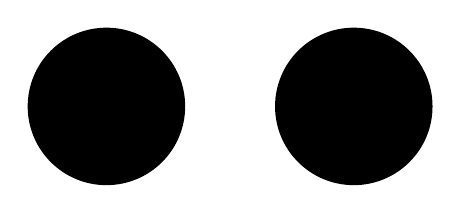
\begin{tikzpicture}[scale=2]

\fill[black] (.5,.5) circle(5mm);
\fill[black] (pi*.5+.5,.5) circle(5mm);
\end{tikzpicture}&
 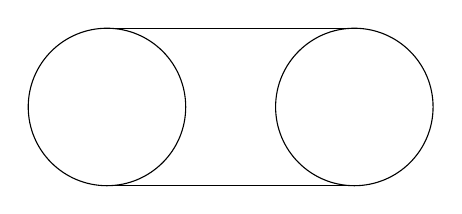
\begin{tikzpicture}[scale=2]

\draw[black] (.5,.5) circle(5mm);
\draw[black] (pi*.5+.5,.5) circle(5mm);
\draw (.5,1) -- (pi*.5+.5,1);
\draw (.5,0) -- (pi*.5+.5,0);
\end{tikzpicture}\\
$\bun{\Omega}$ &$\ext(D \bun{\Omega})$
\end{tabular}
\end{center}
\caption{The extended support for the indicator function of a union of two balls.}
\label{fig:twoBalls}
\end{figure}


\subsection{Support stability}
In this section, we prove that the support of $\ulaw$ is stable around the extended support \eqref{eq:ext_spt_cvx_sets}, i.e.  its support is contained inside some neighborhood of $\ext(Df)$, 
whenever $\la$ and $ \normLdeux{w}/\la$ are sufficiently small.
We begin by proving some properties of the level sets.
\begin{prop}\label{prop:L1_props}
The following statements are true.
\begin{itemize}
\item[(i)] There exists $\al_0,\la_0,L >0$ such that $P(E)\leq L$ for all $E\in \FFlaw$ and $(\la,w)\in D_{1,\sqrt{\cD}/4}$.
\item[(ii)] There exists $R>0$ such that $E_{\la,w}\subset B(0,R)$ for all $\Elaw\in \FFlaw$ with $(\la,w)\in D_{1,\sqrt{\cD}/4}$.
\end{itemize}
\end{prop}
\begin{proof}

To prove (i), 
recall from the discussion in Section \ref{sec:dual_cert_cvx_sets} that $\norm{v_{\la,0}}_{L^2} \leq \norm{\voo}_{L^1}$.
So, for all $E\in\FFlaw$ with $(\la,w)\in D_{1,\sqrt{c_2}/4}$,
 \begin{align*}
 P(E) = \pm\int_E \vlaw \leq \frac{\normLdeux{w}\abs{E}^{1/2}}{\la}+ \norm{v_{\la,0}}_{L^1}
 \leq \frac{ P(E)}{4}  + \norm{\voo}_{L^1}.
 \end{align*}

The proof of (ii) is very similar to the proof of Lemma \ref{lem:largeball}. We first show that there exists $R>0$ such that $E_{\la,w}\cap B(0,R)\neq \emptyset$ for all $\Elaw\in\FFlaw$ with $(\la,w)\in D_{1,\sqrt{c_2}/4}$: let $R$ be such that $B(0,R)\supset \Omega$. For a contradiction, suppose that $\emptyset\neq E_{\la,w}\subset B(0,R)^c$. Then, since $v_{\la,0} = 0$ on $\Omega^c$, we have that
$$
P(E_{\la,w}) = \int_{E_\la,w}(v_{\la,w} - v_{\la,0})  \leq \frac{\norm{w}_{L^2} \abs{E_{\la,w}}^{1/2}}{\la}< \frac{P(E_{\la,w})}{4},
$$ 
which is impossible if $P(E_{\la,w}) > 0$. So, $E_{\la,w}\cap B(0,R)\neq \emptyset$ if $\Elaw\neq\emptyset$. Finally, since by (i), there exists $L>0$ such that $P(\Elaw)\leq L$ for all $(\la,w)\in D_{1,\sqrt{\cD}/4}$,  it follows that $\Elaw\subset B(0,R+L)$.
 
 
\end{proof}


When the source condition is not satisfied,  Proposition \ref{prop:weak_reg} cannot be applied directly to the level sets of $\ulaw$.  However, even if the source condition does not hold, there may still be a subset of $V$ of $\RR^2$ for which
$$
\lim_{\la\to 0}\norm{v_{\la,0}-\voo}_{L^2(V)}= 0.$$ In this case, one can argue along the lines of Proposition \ref{prop:weak_reg} to deduce that  there is still weak regularity on a subset of $\partial E$.  Note that for  characteristic functions on unions of convex sets as described in Section \ref{sec:dual_cert_cvx_sets}, we can let $V=\RR^2 \setminus \ext(Df)$ since $v_{\la,0} = \voo$ on $\RR^2\setminus \ext(Df)$. The precise regularity statement is given in the following proposition.
\begin{prop}\label{prop:weak_reg_partial}
Let $V\subset \RR^2$ be an open set. Suppose that
$$
\lim_{\la\to 0}\norm{v_{\la,0}-\voo}_{L^2(V)} = 0.
$$
Then, there exists $r_0>0$ such that for all $r\in [0, r_0]$ and $\Elaw\in\FFlaw$ with $(\la,w)\in D_{1,\sqrt{\cD}/4}$, if $x\in \partial \Elaw$ is such that $B(x,r_0)\subseteq V$, then
\begin{equation*}
 \frac{\abs{B(x,r)\cap \Elaw}}{\abs{B(x,r)}}\geq \frac{1}{16}\qandq \frac{\abs{B(x,r)\setminus \Elaw}}{\abs{B(x,r)}} \geq \frac{1}{16}.
\end{equation*}
\end{prop}

\begin{thm}\label{thm:union_cvx_sets}
  Let $\Omega$ be a union of convex sets which satisfies the assumptions of Section~\ref{sec:dual_cert_cvx_sets}. %Then the conclusions of Theorem~\ref{thm:spt_stability} hold.
    Let $\{w_n\}_{n\in\NN}$, $\{\la_n\}_{n\in\NN}$ be sequences such that $w_n\in \LDD$, $\la_n\to 0^+$, and ${\normLdeux{w_n}}/{\la_n}\leq \sqrt{\cD}/4$. .
  Then, up to a subsequence, for a.e.\ $t\in \RR$,
  \begin{align}\label{eq:limtbis}
    &\lim_{n\to+\infty} \abs{\Un{t}\Delta \F{t}} =0,\qandq \\
    &\begin{cases}
   \lim_{n\to+\infty} \partial \Un{t}=\partial \F{t}, & \mbox{ if $0<t\leq 1$}\\
   \limsup_{n\to+\infty}  \partial \Un{t}\subseteq \partial \Omega & \mbox{otherwise,}\label{eq:limtter}
\end{cases}
\end{align}
where the last limits holds in the sense of Hausdorff convergence.

If additionally, ${\normLdeux{w_n}}/{\la_n}\to 0$ as $n\to +\infty$, the full sequence satisfies
\begin{equation}\label{eq:suppliminfsupsquare}
  \supp(Df)\subseteq \liminf_{n\to +\infty} \supp(D\un) \subseteq \limsup_{n\to+\infty} \supp(D\un)\subseteq \ext(Df).
\end{equation}

\end{thm}
\begin{proof}
  
  By Proposition~\ref{prop:L1_props} (ii), the level sets $\Un{t}$ are included in some ball $B(0,R)$. So, by the same argument as in Theorem~\ref{thm:spt_stability}, $\partial \F{t}\subseteq\liminf_{n'\to+\infty} \partial\Unp{t}$ and~\eqref{eq:limtbis} holds.

  Now, we prove $\limsup_{n'\to+\infty} \partial\Unp{t}\subseteq \partial \Omega$. Let $(x_{n'})_{n'\in\NN}$ be a sequence in $\RR^2$ such that (up to an additional extraction) $x_{n'}\to x\in \RR^2$, and we assume by contradiction that $x\notin  \partial \Omega$. We let 
  \begin{equation*}
    V\eqdef \enscond{y\in \RR^2}{\dist(y,\partial \Omega)>r_1},
  \end{equation*}
  where $r_1>0$ is such that $r_1<\dist(x,\partial \Omega)$. We observe that $V$ is open, $x\in V$ and $\lim_{n'\to+\infty} \norm{v_{n'}-\voo}_{L^2(V)} = 0$.

  Applying Proposition~\ref{prop:weak_reg_partial}, we obtain for $n'$ large enough and $r>0$ small enough, 
\begin{equation*}
  \abs{B(x_{n'},r)\cap \Unp{t}}\geq \frac{1}{16}\abs{B(x_{n'},r)},\qandq \abs{B(x_{n'},r)\setminus \Unp{t}} \geq \frac{1}{16}\abs{B(x_{n'},r)},
\end{equation*}
and we conclude, passing to the limit as in the proof of Theorem~\ref{thm:spt_stability} that $x\in \partial\F{t}\subseteq \partial \Omega$, which contradicts the hypothesis. Hence $x\in\partial\Omega$, and $\limsup_{n'\to+\infty} \partial\Unp{t}\subseteq \partial \Omega$. Equation~\eqref{eq:limtter} follows since $\partial\F{t}=\partial \Omega$ for $0<t\leq 1$.


It remains to prove $ \limsup_{n\to+\infty} \supp(D\un)\subseteq \ext(Df)$. The proof is quite similar to the proof presented for Theorem \ref{thm:spt_stability} and we merely sketch it for brevity.
We let $x_{n}\to x\in \RR^2$, where $x_n\in \partial E_n$ for some $E_n\in \FFn$ and we assume by contradiction that $x\notin \ext(Df)$. Arguing as  above, and using the compactness property provided by Proposition~\ref{prop:L1_props}, we see that $x\in \partial E$ where $E$ is the limit of $E_n$ (up to an extraction, for the $L^1$ topology).

To conclude, we need to prove that $E\in \FFoo$, as in~\eqref{lsc_perim}. The $L^2$ convergence of 
$v_{\la_n,w_n}$ towards $v_{0,0}$ was applied to prove equation (\ref{lsc_perim}), but in fact, $L^1$ convergence $v_{\la_n,0}$ is sufficient:
Note that by (i) of Proposition \ref{prop:L1_props}  and the isoperimetric inequality, there exists $C$ such that $\abs{E_n}\leq C^2$ for all $n$. Then by letting $E_n\triangle E = (E_n\setminus E) \cup (E\setminus E_n)$,
\begin{align*}
\abs{\int_{E_n} v_{\la_n,w_n} -\int_E \voo}&\leq \abs{ \int_{E_n} v_{\la_n,w_n} - \int_{E_n} \voo} +\abs{ \int_{E_n} \voo - \int_E \voo }\\
&\leq \norm{v_{\la_n,0}  - \voo}_{L^1} +\frac{C \normLdeux{w_n}}{\la_n} + \int_{E_n\triangle E}\voo \to 0,
\end{align*}
by the $L^1$ convergence of $(v_{\la,0})$ and the absolute continuity of the Lebesgue integral.
As a result,  $E\in \FFoo$, hence $x\in \partial E\subseteq \ext(Df)$, and $\limsup_{n\to+\infty} \supp(D\un)\subseteq \ext(Df)$.
\end{proof}
